% VUT FIT MITAI
% MSZ 2021/2022
% Author: Vladimir Dusek
% Login: xdusek27

%%%%%%%%%%%%%%%%%%%%%%%%%%%%%%%%%%%%%%%%%%%%%%%%%%%%%%%%%%%%%%%%%%%%%%%%%%%%%%%%

% Path to figures
\graphicspath{{upa/ziskavani_znalosti_z_dat/figures}}

%%%%%%%%%%%%%%%%%%%%%%%%%%%%%%%%%%%%%%%%%%%%%%%%%%%%%%%%%%%%%%%%%%%%%%%%%%%%%%%%

\chapter{UPA~--~Získávání znalostí z dat (pojem znalost; typické zdroje dat; základní úlohy získávání znalostí; analytické projekty a proces získávání znalostí z dat).}

%%%%%%%%%%%%%%%%%%%%%%%%%%%%%%%%%%%%%%%%%%%%%%%%%%%%%%%%%%%%%%%%%%%%%%%%%%%%%%%%

\section{Zdroje}

\begin{compactitem}
    \item Má DP.
    \item \path{10-ziskavani_znalosti.pdf}
    \item \path{UPA_2019-11-26.mp4}
    \item \path{UPA_2019-12-03.mp4}
\end{compactitem}

%%%%%%%%%%%%%%%%%%%%%%%%%%%%%%%%%%%%%%%%%%%%%%%%%%%%%%%%%%%%%%%%%%%%%%%%%%%%%%%%

\section{Úvod a kontext}

\begin{compactitem}
    \item Získávání znalostí z databází (dat) je proces extrahování a objevování vzorů ve velkých datových souborech na pomezí strojového učení, statistiky a databázových systémů.

    \item Cílem je získat informace dopředu neznámé a potenciálně užitečné (\textbf{znalost}) a transformovat je do srozumitelné struktury pro další použití.
\end{compactitem}

%%%%%%%%%%%%%%%%%%%%%%%%%%%%%%%%%%%%%%%%%%%%%%%%%%%%%%%%%%%%%%%%%%%%%%%%%%%%%%%%

\section{Proces získávání znalostí z dat}

\begin{compactitem}
    \item Celý proces získávání znalostí je zobrazen na obrázku dále. Jedná se o iterativní sekvenci kroků, které jsou představeny v~následujícím výčtu.
\end{compactitem}

\begin{compactenum}
    \item \textbf{Datové čištění}~--~Odstranění šumu, nekonzistencí, neúplností a dalších znaků dat nízké kvality.

    \item \textbf{Datové integrace}~--~Kombinace několika různých datových zdrojů. Proces čištění a integrace bývá typicky prováděn v~jednom kroku jako forma předzpracování (příprava dat). Výsledky tohoto kroku pak jsou ukládány do datového skladu.

    \item \textbf{Výběr}~--~Selekce relevantních dat z~datového skladu pro konkrétní dolovací úlohu.

    \item \textbf{Datové transformace}~--~Transformace dat do potřebné podoby pro konkrétní dolovací algoritmus.

    \item \textbf{Dolování z~dat}~--~Hlavní krok ve kterém jsou použity statistické metody či algoritmy strojového učení pro získávání nových dat (datových vzorů).

    \item \textbf{Vyhodnocení}~--~Vyhodnocení a identifikování datových vzorů, které mohou představovat novou znalost.

    \item \textbf{Prezentace}~--~Předávání a prezentování získaných znalostí uživatelům pomocí vhodných vizualizačních technik.
\end{compactenum}

\begin{figure}[H]
    \centering
    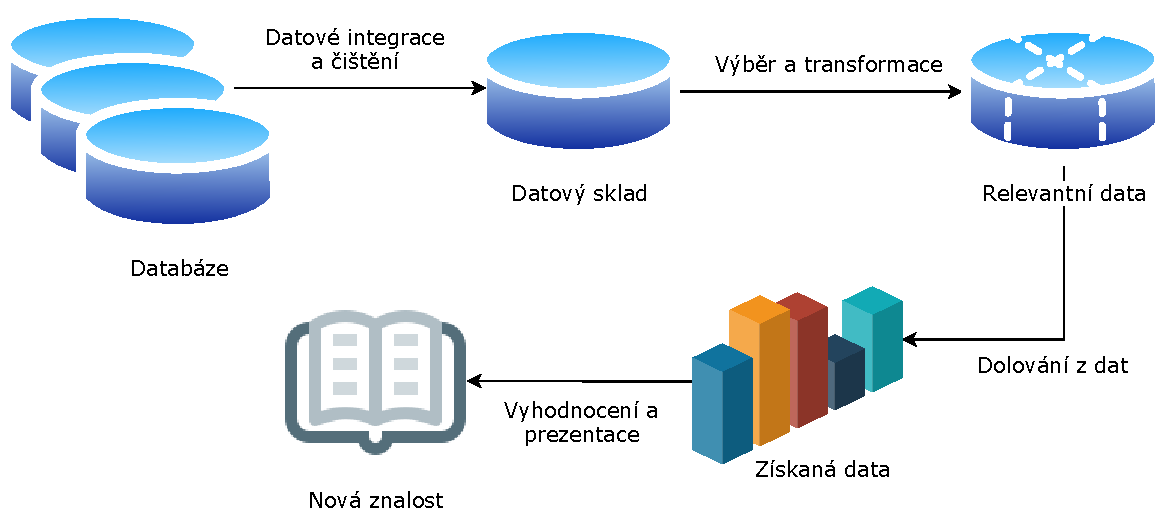
\includegraphics[width=1\linewidth]{knowledge_discovery_diagram.pdf}
    \caption{Fáze procesu získávání znalostí z~databází. V~diagramu je možné se vracet zpět a jednotlivé fáze libovolně revidovat a opakovat (např. zvolit jiné parametry dolovacího algoritmu pro získání lepších výsledků).}
\end{figure}

\subsection{Model CRISP}

\begin{compactitem}
    \item Model CRISP (\textit{CRoss-Industry Standard Process for Data Mining}) je formální, teoretický model, popisující proces získávání znalostí z databází.

    \item Časté jsou návraty mezi fázemi modelu.
\end{compactitem}

\begin{compactenum}
    \item \textbf{Pochopení kontextu}~--~Cílem je dozvědět se co nejvíce o kontextu řešeného problému (pochopení dané problematiky).

    \item \textbf{Pochopení dat}~--~Cílem je dozvědět se o dostupných/potřebných datech co nejvíce (popis, prozkoumání a zhodnocení kvality dat).

    \item \textbf{Příprava dat}~--~Cílem je připravit data pro aplikaci dolovacího algoritmu (výběr, čištění, integrace, transformace).

    \item \textbf{Modelování}~--~Cílem je vytvořit model připravených dat.

    \item \textbf{Zhodnocení}~--~Cílem je zhodnotit dosažené výsledky a další postup.

    \item \textbf{Použití}~--~Cílem je stanovit strategie použití výsledků a naplánování kroků.
\end{compactenum}

\begin{figure}[H]
    \centering
    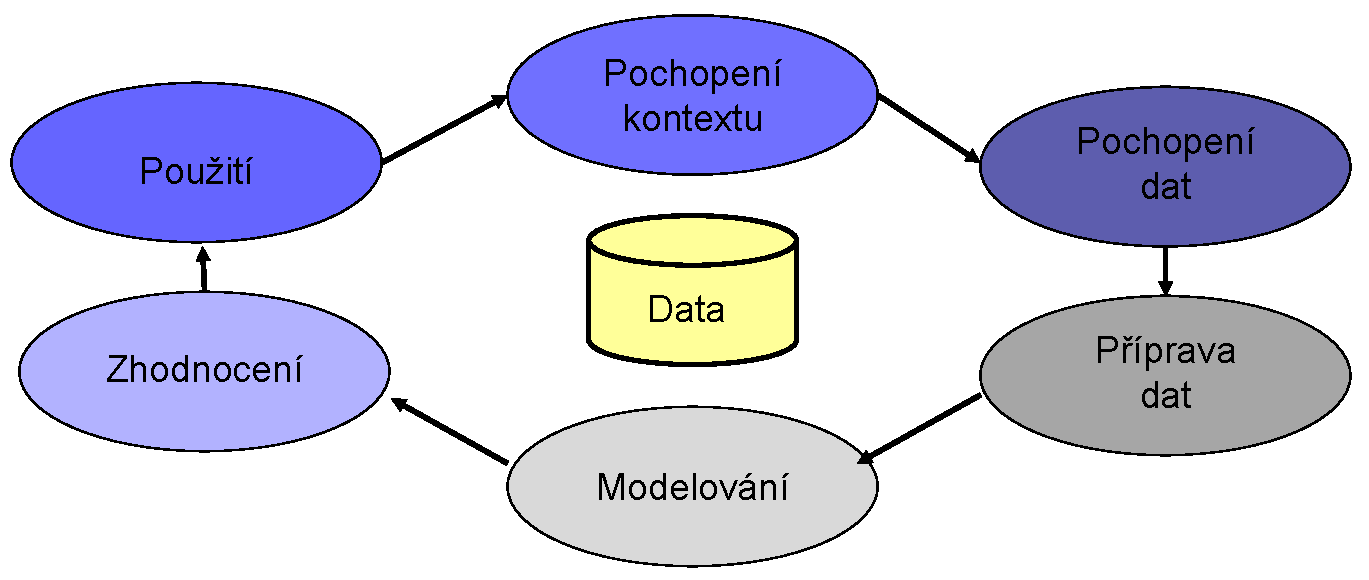
\includegraphics[width=0.75\linewidth]{crisp.pdf}
    \caption{Model CRISP.}
\end{figure}

%%%%%%%%%%%%%%%%%%%%%%%%%%%%%%%%%%%%%%%%%%%%%%%%%%%%%%%%%%%%%%%%%%%%%%%%%%%%%%%%

\section{Analytické (data mining) projekty}

\begin{compactitem}
    \item Analogie bežných softwarových projektů.
    \item Zadavatel: vlastní organizace / jiná organizace.
    \item Řešitel: datoví analytici (+ programátoři), doménoví experti.
    \item Vstupy: \begin{compactitem}
        \item Vymezení problému k řešení pro rozhodování na základě dat (\textit{Data-Driven Decision making}).
        \item Dostupná data (interní, externí).
    \end{compactitem}
    \item Výstup: využitelná znalost -- model dat, vzory v datech, profily atd.
    \item Technologie: \begin{compactitem}
        \item Programování s využitím knihoven (např. Python + Scikit Learn).
        \item Prostředí nějakého dolovacího nástroje (např. Rapid Miner).
    \end{compactitem}
\end{compactitem}

%%%%%%%%%%%%%%%%%%%%%%%%%%%%%%%%%%%%%%%%%%%%%%%%%%%%%%%%%%%%%%%%%%%%%%%%%%%%%%%%

\section{Typické zdroje dat}

\begin{compactitem}
    \item Relační databáze
    \item Datové sklady -- Modelován jako multidimenzionální datová kostka. Zpřístupnění pomocí OLAP operací.
    \item Transakční databáze -- Soubor / tabulka jehož každý záznam reprezentuje obchodní transakci.
    \item Dokumenty (textové / multimediální) -- Datový soubor.
    \item Proudy dat (senzory, kamery, \dots).
    \item Velmi rozsáhlá data (\textbf{Big Data}) \begin{compactitem}
        \item vysoký objem (\textit{volume}),
        \item vysoká rychlost vzniku (\textit{velocity}),
        \item rozličnost zdrojů, typů, formátů (\textit{variety}),
        \item věrohodnost, nejistá vlivem nekonzistence, neúplnosti (\textit{veracity}).
    \end{compactitem}
\end{compactitem}

%%%%%%%%%%%%%%%%%%%%%%%%%%%%%%%%%%%%%%%%%%%%%%%%%%%%%%%%%%%%%%%%%%%%%%%%%%%%%%%%

\section{Úlohy získávání znalostí}

\begin{compactitem}
    \item Typy dolovacích úloh můžeme rozdělit do dvou základních skupin:

    \begin{compactitem}
        \item \textbf{Deskriptivní}~--~Deskriptivní úlohy charakterizují obecné vlastnosti a vztahy v~analyzovaných datech, které mohou pomoci učinit lepší rozhodnutí (korelační analýza, dolování frekventovaných vzorů, asociační analýza, shluková analýza, analýza odlehlých hodnot). Např. časté společné nákupy zboží při analýze nákupního košíku.

        \item \textbf{Prediktivní}~--~Prediktivní úlohy provádí předpověď budoucího chování na základě analýzy současných dat (klasifikace, regrese). Např. předpověď chování nového zákazníka na základě dosavadního chování zákazníků.
    \end{compactitem}
\end{compactitem}

\subsection{Frekventované vzory}

\begin{compactitem}
    \item Frekventované vzory (\textit{frequent patterns}) jsou vzory, které se v~datech vyskytují často. Jejich dolování vede objevování zajímavým asociací a korelací v~datech.

    \item Existuje mnoho druhů frekventovaných vzorů, včetně frekventovaných množin, frekventovaných podsekvencí (sekvenční vzory) a frekventovaných podstruktur.

    \item Frekventovaná množina obvykle označuje množinu položek, které se často vyskytují společně v~souboru transakčních dat (např. mléko a chléb, které mnoho zákazníků mnohdy kupuje společně).

    \item Frekventované podsekvence značí události, které často nastávají po sobě (např. zákazníci mají tendenci kupovat digitální fotoaparát a poté paměťovou kartu).

    \item Substruktura se může vyskytovat v~datech, která mají strukturní formu (např. grafy, stromy nebo mřížky).
\end{compactitem}

\subsection{Asociační analýza}

\begin{compactitem}
    \item Asociační analýza (\textit{association rule learning}) je metoda nalézání asociačních pravidel spojujících zároveň se vyskytující atributy (např. události, položky atd.) ve zkoumaných datech.

    \item Typickým použitím je analýza nákupního košíku, tj. zkoumání, které položky jsou často nakupovány společně.

    \item Příkladem takového asociačního pravidla může být
    \begin{equation}
        kupuje(X, pocitac) \rightarrow kupuje(X, monitor)
    \end{equation}
    kde $X$ je proměnná reprezentující zákazníka. Pravidlo říká, že pokud si zákazník koupí počítač, pravděpodobně si koupí i monitor.
\end{compactitem}

\subsection{Klasifikace}

\begin{compactitem}
    \item Klasifikace (\textit{classification}) je forma prediktivní úlohy, kdy je novým datovým vzorům přiřazováno předem známé kategoriální označení tříd (zařazování dat do skupin na základě různých aspektů).

    \item Taková analýza pomáhá lépe porozumět datům jako celku.

    \item Z~hlediska strojového učení se jedná o~úlohu učení s~učitelem.

    \item Klasifikátor je nejprve třeba naučit na označené trénovací datové sadě. Až poté je možné, aby klasifikátor predikoval přiřazení třídy novým datům.

    \item Možné využití klasifikace: \begin{compactitem}
        \item Klasifikace potenciálních zákazníků banky na základě rizikovosti na ty, kterým je vhodné poskytnout úvěr a na ty kterým ne.

        \item Klasifikace e-mailů~--~Rozhodnout, zda se jedná o~spam či nikoliv.

        \item Stanovení lékařské diagnózy na základě výsledků různých vyšetření.

        \item Cílení marketingu~--~Vyhodnotit kterému uživateli zobrazit jakou reklamu.
    \end{compactitem}

    \item Mezi běžné klasifikační metody patří:

    \begin{compactitem}
        \item klasifikátor k-nejbližších sousedů,

        \item Bayesovská (naivní) klasifikace a Bayesovské sítě,

        \item rozhodovací stromy,

        \item SVM (\textit{Support Vector Machine}),

        \item klasifikace pomocí neuronových sítí.
    \end{compactitem}
\end{compactitem}

\subsection{Regrese}

\begin{compactitem}
    \item Regrese (\textit{regression}) je prediktivní úloha, ve které se na základě znalosti jistých atributů predikuje hodnota jiného (cílového) atributu.
    \item Narozdíl od klasifikace, není cílový atribut kategorický, nýbrž numerický (má spojitý charakter). \item Možné využití regrese: \begin{compactitem}
        \item Určení výše platu pracovníka na základě znalostí jeho dalších vlastností.

        \item Predikce očekávané pooperační délky života pacientů trpících rakovinou.

        \item Predikce výšky dítěte.

        \item Predikce vývoje ceny komodity.
    \end{compactitem}

    \item Pro účely regrese lze využít některé klasifikační algoritmy (neuronové sítě, k-nejbli\-žších sousedů, SVM) rozšířené o~predikování spojité veličiny a nebo regresní analýzu. Regresní analýza je matematická metoda hledání závislostí mezi atributy. V~podstatě jde o~aproximaci trénovacích dat vhodnou funkcí (regresní funkce).

    \item Jsou rozlišovány různé typy: \begin{compactitem}
        \item \textbf{Jednoduchá lineární regrese}~--~Cílový atribut závisí na jednom dalším atributu lineárně.

        \item \textbf{Vícenásobná lineární regrese}~--~Cílový atribut závisí na několika dalších atributech lineárně.

        \item \textbf{Nelineární regrese}~--~Cílový atribut závisí na dalších atributech nelineárně.
    \end{compactitem}
\end{compactitem}

\subsection{Shluková analýza}

\begin{compactitem}
    \item Na rozdíl od klasifikace nejsou při shlukové analýze (\textit{clustering}) předem známy třídy rozdělení dat.

    \item Proces shlukování se sám snaží data rozdělit do přirozených skupin (shluků).

    \item Vytvořené shluky pravděpodobně odrážejí nějaký fenomén v~datech, který způsobuje, že některé instance jsou si navzájem podobnější než jiné.

    \item Vytvořené shluky pravděpodobně odrážejí nějaký fenomén v~datech, který způsobuje, že některé instance jsou si navzájem podobnější než jiné.

    \item Existují různé způsoby, jak lze vyjádřit výsledek shlukování:

    \begin{compactitem}
        \item Identifikované shluky tvoří disjunktní množiny. Každá instance patří pouze do jednoho shluku a každý shluk obsahuje alespoň jednu instanci.

        \item Identifikované shluky se mohou překrývat. Každá instance může patřit do několika shluků.

        \item Identifikované shluky se překrývají a každá instance patří do každého shluku s~určitou pravděpodobností.

        \item Identifikované shluky tvoří hierarchickou strukturu. Na nejvyšší úrovni je hrubé rozdělení instancí do shluků a každý shluk je dále upřesněn, v~krajním případě až na jednotlivé instance.
    \end{compactitem}

    \item Za základní algoritmus shlukování je považován algoritmus \textbf{k-means} (\textit{k-means clustering}). Data rozděluje do shluků, které tvoří disjunktní množiny a počet shluků musí být předem zadán ($k$). Na začátku je náhodně vybráno $k$ počátečních bodů, které představují počáteční středy shluků. Všechny datové body jsou přiřazeny do shluků podle vzdálenosti k~nejbližšímu středu. Poté je vypočtena střední hodnota bodů v~každém shluku, aby se vytvořil nový střed shluku. Takto algoritmus iterativně pokračuje, dokud dochází ke změnám ve shlucích.
\end{compactitem}

\subsection{Analýza odlehlých hodnot}

\begin{compactitem}
    \item Cílem analýzy odlehlých hodnot (\textit{outlier detection}) je nalezení extrémních hodnot, které se výrazně liší od ostatních.

    \item Takové datové objekty se nazývají odlehlé (anomálie). Možné využití analýzy odlehlých hodnot: \begin{compactitem}
        \item Odhalení podezřelého chování na záběrech z~bezpečnostních kamer.

        \item Detekce vadných kusů při výrobě.

        \item Odhalení platby odcizenou platební kartou.

        \item Detekce chyb měření.
    \end{compactitem}

    \item Pro tyto účely je možné využít statistické metody. Nejprve jsou v~datech hledány pravděpodobností rozdělení, které stojí za generováním dat. Datové vzory, pro které je velmi nepravděpodobné, že byly vygenerovány tímto vybraným rozdělením, jsou prohlášeny za odlehlé hodnoty.

    \item Dále je možné využít některé upravené klasifikační metody, jako jsou algoritmus k-nejbližších sousedů, neuronové sítě a SVM. Také je možné využít některé shlukovací algoritmy, které dokáží přirozeně detekovat hodnoty, které se výrazně liší od ostatních a nepřiřadit je do žádného shluku. Jedná se o~tzv. metody shlukování založené na hustotě.
\end{compactitem}
